\documentclass[11pt]{ctexart}         %编辑中文文档
\usepackage{amsmath,amsfonts,amssymb} %数学工具包
\usepackage[margin=1in]{geometry}     %页面设置,边距,页幅大小等
\usepackage{enumerate}                %有序列表工具包
%\usepackage{hyperref}                 %方便设置超链接
\usepackage{fancyhdr}                 %设置页眉页脚
\usepackage{float}                    %设置图片环绕样式
\usepackage{graphicx}                 %插入图片
\usepackage{color}
\usepackage{xcolor}
\usepackage{adjustbox}
\usepackage{pifont}
\usepackage{extarrows}
\usepackage{enumitem}
\usepackage{setspace}
\usepackage{subfigure}

\CTEXsetup[format={\Large\bfseries}]{section} %设置section标题左对齐,挺迷的
\usepackage[
	pdfstartview=FitH,
	CJKbookmarks=true,
	bookmarksnumbered=true,
	bookmarksopen=true,
	colorlinks,
	pdfborder=001,
	linkcolor=blue,
	anchorcolor=blue,
	citecolor=blue,
]{hyperref}
\hypersetup{hidelinks} %去除目录项以及超链接的方框

\pagestyle{fancy}                     %设置页眉页脚
\fancyhead{}                          %清除默认页眉
\fancyfoot{}                          %清除默认页脚
\fancyhead[L]{\slshape{Convex Optimization}}%设置自定义页眉左侧,slshape表斜体	
\fancyhead[R]{\slshape Chapter4 Convex Problem}	
\fancyfoot[C]{\thepage}
\parindent 0ex %latex首段不缩进,其后段落缩进,\parindent为其后段落缩进的长度
\setlength{\parskip}{1em}  %段落间距
\renewcommand{\baselinestretch}{1.5}  %设置行距
\renewcommand{\vec}[1]{\boldsymbol{#1}}  %设置粗体向量
\newcommand{\tabincell}[2]{\begin{tabular}{@{}#1@{}}#2\end{tabular}}%表格内换行

\newenvironment{myenumerate}{\begin{enumerate}[itemsep=0pt,parsep=0pt,topsep=0pt]}{\end{enumerate}}
\newcommand{\liset}{itemsep=0pt,parsep=0pt,topsep=0pt}
\newcommand{\rebacklinespread}[1][-12pt]{\vspace{#1}}
\newcommand{\oneline}[1][12pt]{\vspace{#1}}
\newcommand{\premise}[1][dom\ f]{\forall\ x,y\in #1,\ \theta\in [0,1]}
\newcommand{\linearcombine}[2]{\theta #1+(1-\theta)#2}
\newcommand{\ii}{\,\in\,}
\newcommand{\dom}[1]{$dom\ #1$}
\newcommand{\rs}[2][R]{#1^{#2}} %Rspace or matrix space
\newcommand{\rl}[2][R]{#1_{#2}} %Rlimit or matrix space
\newcommand{\rls}[3][R]{#1_{#2}^{#3}} %R limit space or matrix limit space

\newcommand{\trans}[1]{#1^T#1} %transpose
\newcommand{\ftrans}[1]{\left(#1\right)^T#1} %fraction transpose

\newcommand{\ba}[1]{\begin{align*}#1\end{align*}}
\newcommand{\bc}[1]{\begin{cases}#1\end{cases}}
\newcommand{\bcenter}[1]{\begin{center}#1\end{center}}
\newcommand{\li}[3][例]{
	#1:#2\\ 
	\phantom{#1:}\begin{minipage}[t]{0.9\linewidth}%注意这里phantom和minipage之间不能换行
	\setlength\parskip{12pt}
	#3
	\end{minipage}
	\oneline}
\newcommand{\sune}{\parbox{1em}{$ \Rightarrow $\\ [-10pt] $ \nLeftarrow $}} % Sufficiently unnecessary
\newcommand{\usne}{\parbox{1em}{$ \nRightarrow $\\ [-10pt] $ \Leftarrow $}} % unsufficiently necessary
\newcommand{\paint}[2][red]{{\color{#1}#2}} %着色
\newcommand{\VV}[1]{\Vert #1 \Vert}


\begin{document}
\hrule height 4pt
\begin{Large}
	\textbf{Essence of the lecture (19/21/22/23/24)}\\
\end{Large}
\begin{large}
	\textbf{凸问题:} 
\end{large}
\vspace{-16pt}
\begin{itemize} \setlength{\itemsep}{0pt}
	% 使用\displaystyle来解决行内时bigcap变形
	\item 非凸、非拟凸问题的松弛(零范数的松弛)
	\item 广义凸问题及相关定义
	\item 问题的等价变换
	\item 狭义凸问题
	\item 凸问题的性质:局部最优=全局最优,目标函数可微情况下的最优解
\end{itemize}
% 设置hrule的宽度为4pt
\hrule height 4pt

\textbf{零范数的松弛:}\\
在一维条件下,零范数是拟凸函数(非凸),在$ n\geq 2 $情况下,零范数非拟凸,此时主要有两种松弛方法。
\rebacklinespread
\begin{itemize}\setlength{\itemsep}{0pt}
	\item 松弛为$l_1$范数,该函数为凸函数
	\item 松弛为$ log(ax^2+1) $,该函数非凸,但是是拟凸函数
	\begin{figure}[h]
		\centering
		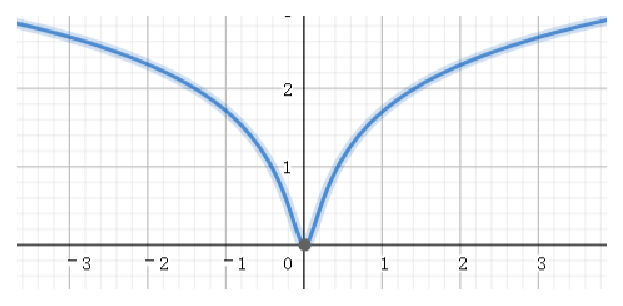
\includegraphics{imgs/logax.eps}
		\caption{$ f(x)=log(ax^2+1),a\to +\infty$时整体趋近零范数,拟凸函数}
	\end{figure}
	\rebacklinespread
\end{itemize}
\rebacklinespread
广义凸问题:凸目标,凸集约束\\
一般优化问题的描述:
\rebacklinespread
\begin{align*}
	&\min\ f_0(x)\\& s.t.\ 
	\begin{array}[t]{ll}% 注意一定要加上{l/c/r}
		f_i(x)\leq 0\quad &i=1,\dots,m\\
		h_i(x)=0\quad &i=1,\dots,p
	\end{array}
\end{align*}
x称为优化变量(optimization variable),$ f_0 $称为目标函数、损失函数、效用函数,$ f_i(x)\leq 0 $称为不等式约束(inequality constraint),$ h_i(x)=0 $称为等式约束(equality constraint),$ m=p=0 $时为无约束(unconstrained)问题

\newpage
\textbf{概念定义(注意inf可以对应min):}
\rebacklinespread
\begin{description}[itemsep=0pt]
	\item[优化问题的域(domain):] D=$\displaystyle\bigcap_{i=0}^m dom\ f_i \ \cap\ \displaystyle\bigcap_{i=1}^p dom\ h_i$
	\item[可行解集(feasible set):] $ X_f=\{x\mid x\in D,\ f_i(x)\leq 0,i=1,\dots,m,\ h_i(x)=0,i=1,\dots,p\}$
	\item[最优值(optimization value):] $ p^*=\inf\ \{f_0(x)\mid x\in X_f\}$,若$ X_f=\oslash,\ p^*=+\infty $
	\item[最优解(optimization point/solution):] 若$ x^* $可行,且$ f_0(x^*)=p^* $,称$ x^* $为最优解
	\item[$\varepsilon$次优解集($\varepsilon$-suboptional set):] $ X_{\varepsilon}=\{x\mid x\in X_f,\ f_0(x)\leq p^*+\varepsilon\} $
	\item[局部最优解(locally optional):] $ f_0(x)=\inf\ \left\{f_0(z)\mid 
	\begin{array}[c]{l}
		f_i(x)\leq 0,i=1,\dots,m\\
		h_i(z)=0,i=1,\dots,p\\
		\Vert z-x\Vert\leq R
	\end{array}
	\right\} $,解集为$ X_{loc} $
\end{description}

\textbf{不等式约束采用$ \leq $而非<的原因}\\
若$ x\in X_f,\ f_i(x)=0 $,则$ f_i(x)\leq 0 $为活动(active)约束\\
若$ x\in X_f,\ f_i(x)<0 $,则$ f_i(x)\leq 0 $为非活动(inactive)约束\\
而所有的<约束都可以转化为$ \leq $约束\\
例如 money<100$\Rightarrow-\vert log(100-money)\vert\leq 0$

\textbf{问题的等价变换}\\
\li{Box Constraint}{
	\[ l_i\leq x\leq u_i \Rightarrow 
	\begin{cases}
		l_i-x_i\leq 0\\
		x_i-u_i\leq 0
	\end{cases}
	\]}

\li{将问题的量纲做标准化}{
	\vspace{-48pt}
	\begin{align*}
		&\min\ \alpha_0\,f_0(x)\\
		& s.t.\ 
		\begin{array}[t]{ll}% 注意一定要加上{l/c/r}
			\alpha_i\,f_i(x)\leq 0\quad &i=1,\dots,m\\
			\beta_i\,h_i(x)=0\quad &i=1,\dots,p
		\end{array}
	\end{align*}
}

\li{利用函数进行等价变换}{
	\begin{center}
		\begin{tabular}[t]{|c|c|c|}
			\hline
			$ \psi_0$&$ R\to R $& 单增 \\
			\hline
			$ \psi_1,\dots,\psi_m$&$ R\to R $& $ \psi_i(u)\leq 0 \Leftrightarrow u\leq 0 $ \\
			\hline
			$ \varrho_1,\dots,\varrho_p $& $ R\to R $&$ \varrho_i(u)=0\Leftrightarrow u=0 $ \\
			\hline
		\end{tabular}
	\end{center}
	\vspace{-24pt}
	\begin{align*}
		&\min\ \psi_0\,(f_0(x))\\
		& s.t.\ 
		\begin{array}[t]{ll}% 注意一定要加上{l/c/r}
			\psi_i\,(f_i(x))\leq 0\quad &i=1,\dots,m\\
			\varrho_i\,(h_i(x))=0\quad &i=1,\dots,p
		\end{array}
	\end{align*}
	\bcenter{如 $ \min \Vert Ax-b\Vert_2\Leftrightarrow\Vert Ax-b\Vert_2^2 $}
}

\li{消除等式约束}{$\{h_i(x)=0,i=1,\dots,p\}$看作一组方程,$ X=\varrho(Z),\ Z\in R^k,\ \varrho:\ R^k\to R^n $
	\rebacklinespread
	\begin{align*}
		&\min\ f_0(\varrho(x))\quad \Rightarrow\quad  X^*=\varrho(Z^*)\\
		& s.t.\ 
		\begin{array}[t]{ll}% 注意一定要加上{l/c/r}
			f_i(\varrho(x))\leq 0\quad &i=1,\dots,m
		\end{array}
	\end{align*}
}

\li{消除线性等式约束}{在线性等式约束的情况下,$ h_i(x)=0\Rightarrow Ax-b=0 $\\
	此时若方程无解,则问题无解,若A可逆,则$ X=A^{-1}b $\\
	否则可将等式约束化为$ X=FZ+X_0 $,FZ在A的零空间,即将求解n维的X化为求解n-r维的Z(因为初等变换F不改变Z的秩)\\
	\paint{只有在有必要的情况下这样做,有时候会带来麻烦(具体麻烦未提及)}}

\textbf{狭义凸问题:}
\rebacklinespread
\begin{alignat*}{4}%align*还有flalign*都是弹性距离,alignat距离可调
	\min\quad &f_0(x)		&&			 &&\qquad f_0(x)\text{为凸}\\
	s.t.\quad &f_i(x)\leq 0	&&\qquad i=1,\dots,m &&\qquad f_i(x)\text{均为凸}\\
		  &a_i^Tx=b_i	&&\qquad i=1,\dots,p &&\qquad \text{等式约束为仿射函数}
\end{alignat*}

\newpage
\li{引入松弛变量(slack variable)$ s_i $}{
	虽然是一个升维的情况,但是有时可以将问题化为非常特殊的形式更易求解
	\rebacklinespread
	\begin{alignat*}{3}%align*还有flalign*都是弹性距离,alignat距离可调
		\min\quad &f_0(x)		&&\\
		s.t.\quad &s_i\leq 0    &&\\
				  &f_i(x)-s_i=0 &&\qquad i=1,\dots,m \\
				  &a_i^Tx=b_i	&&\qquad i=1,\dots,p 
	\end{alignat*}
}

\textbf{类似有相关问题(max concave $\Leftrightarrow$ min convex)}
\rebacklinespread
\begin{description}
	\item[Quasi-convex optimization] $ f_0 $为拟凸函数,$ f_i,\ h_i $为凸函数
	\item[None-convex optimization] $ f_0 $为凹函数,$ f_i,\ h_i $为凸函数
\end{description}

\li[\textbf{求证}]{\textbf{凸问题的局部最优即为全局最优}}{
	设x不是全局最优,$\exists y\in X_f,\ s.t.\ f_0(y)<f_0(x)$\\
	$\because$ x为局部最优,$\Rightarrow \Vert y-x\Vert_2>R$\\
	令$ z=\linearcombine{y}{x} $,取$ \theta=\dfrac{R}{2\Vert y-x\Vert_2}\in [0,1] $\\[6pt]
	$\therefore$ z为凸组合,$ z\in X_f $且\paint[blue]{$ f_0(z)\leq \linearcombine{f_0(y)}{f_0(x)} $}\\
	$ \Vert z-x\Vert_2=\theta \Vert x-y\Vert_2=\frac{R}{2}<R $,由x局部最优有$ f_0(x)\leq f_0(z) $\\
	由此应该有\paint[blue]{$ f_0(y)<f_0(x)\leq f_0(z) $}  (两条蓝色结论矛盾,因此原假设成立)
}

\li[\textbf{分析}]{\textbf{目标函数可微情况下的最优解}}{
	考虑凸函数的一阶条件:$ f(y)\geq f(x)+\nabla f^T(x)(y-x) $\\
	对于全局最优$ x^* $,此时一定有$ \nabla f^T_0(x^*)(y-x^*)\geq 0 $
}

\li{约束仅为等式约束的情况,$ \min\ f_0(x)\ s.t.\ x\geq 0 $}{
	此时问题仅有$ Ax=b $这一约束条件,由$ Ax^*=b,\ Ay=b \Rightarrow y=x^*+\upsilon,\ \upsilon\in Null(A)$\\
	回代,有$ \nabla f^T(x)\upsilon\geq 0 $\\
	要求对$ \forall\upsilon\in Null(A) \text{均成立}\Rightarrow\bc{\upsilon=0\\ \nabla f(x)\text{与Null(A)正交}}$\\ [6pt]
	第一种情况下,$ x=y $,说明有且仅有一解,$ x=A^{-1}b $
}

\newpage
\li{约束仅为非负约束,$ \min f_0(x)\ s.t.\ x\geq 0 $}{
	即在给定x的情况下,对于$ \forall y \geq 0,\ \nabla f^T(x)(y-x)\geq 0\Rightarrow \nabla f^T(x)y-\nabla f^T(x)x\geq 0$\\
	$ f^T(x)y=\sum a_i x_i $,为了保证对于任意y成立,故$ a_i\geq 0\Leftrightarrow \nabla f(x)\geq 0 $\\
	结合$ x\geq 0 $,有\paint[blue]{$ \nabla f^T(x)x\geq 0 $},又取y=0时,有\paint[blue]{$ \nabla f^T(x)x\leq 0 $}\\ [6pt]
	综上,有$ \nabla f^T(x)= 0 \Rightarrow\bc{x\geq 0\\ \nabla f(x)\geq 0\\ (\nabla f(x))_ix_i=0}$ \paint{(互补条件:Complementarity)}
}

\newpage
\hrule height 4pt
\begin{Large}
	\textbf{Essence of the lecture (25/26/27/28)}\\
\end{Large}
\begin{large}
	\textbf{典型的凸问题:} 
\end{large}
\vspace{-16pt}
\begin{itemize} \setlength{\itemsep}{0pt}
	\item 线性规划
	\item 线性分数规划
	\item 二次规划(二次约束的二次规划)
	\item 半正定规划
	\item 多目标优化
\end{itemize}
% 设置hrule的宽度为4pt
\hrule height 4pt
\textbf{线性规划:}\\
线性规划要求目标和约束均为线性
\rebacklinespread
\begin{description}
	\item[linear program] 线性问题(名词)
	\item[linear programing] 线性问题求解(动词)
\end{description}
\vspace{-24pt}
\begin{align*}
	min\quad &c^Tx+d\\
	s.t.\quad &Gx\leq h,\ Ax=b
\end{align*}
\textbf{线性规划的等价变换}
\rebacklinespread
\begin{alignat*}{4}
	\min\quad&c^Tx+d&&\hspace{7em}\min\quad &&c^Tx^+-c^Tx^-+d\\
	s.t.\quad&Gx+s=h&&\hspace{7em}s.t.\quad &&Gx^+-Gx^-+s=h\\
			 &Ax=b	&&			&&Ax^+-Ax^-=b\\
			 &s\geq 0&&			&&s\geq 0,\ x^+\geq 0,\ x^-\geq 0
\end{alignat*}
\paint{通过这种变换能够将问题化为线性约束以及非负约束,这方便使用函数(linprog)进行求解。}

\newpage
\textbf{线性分数规划(linear fractional programing)}\\
BTW,线性分数函数保凸,是拟凸函数但不是凸函数,例如$ 1/x $
\rebacklinespread
\begin{alignat*}{6}
		(P_0)\qquad&\min\quad &&\dfrac{c^Tx+d}{e^Tx+f}&&\hspace{5em}(P_1)\qquad&&\min\quad &&c^Ty+dz\\
			 &s.t.\quad &&Gx\leq h&&   &&s.t.\quad &&Gy-hz\leq 0\\
			 &			&&Ax=b	  &&   &&		   &&Ax-bz=0\\
			 &			&&e^Tx+f>0&&   &&		   &&e^Ty+fz=1\\
			 &			&&		  &&   &&		   &&z\geq 0
\end{alignat*}
\paint{证明两问题等价的思路:P1的可行解在P2可行,P2的可行解在P1可行,同时二者的值相同}\\
证明:\begin{minipage}[t]{0.9\linewidth}
	\setlength\parskip{12pt}
	1) 若x在$ P_0 $可行,取$ y=\dfrac{x}{e^Tx+f},\ z=\dfrac{1}{e^Tx+f} $
	\rebacklinespread
	\ba{\bc{
			Gy-hz=\dfrac{Gx-h}{e^Tx+f}\leq 0\\[6pt]
			Ay-bz=\dfrac{Ax-b}{e^Tx+f}=0\\[6pt]
			e^Tx+fz=\dfrac{e^Tx+f}{e^Tx+f}=1\\[6pt]
			z>0}\Rightarrow \text{x同时在P1可行,同时目标函数值均为}\ \dfrac{c^Tx+d}{e^Tx+f}}
	2) 若y,z在$ P_1 $中可行\\
	当$ z>0\Rightarrow x=\dfrac{y}{z} $在$ P_0 $可行,且目标函数值均为$ c^Ty+dz $\\
	当$ z=0 $,此时有$ Gy\geq 0,\ Ay=0,\ e^Ty=1 $,设$ x_0 $为$ P_0 $的可行解,找到射线$ x=x_0+ty,\ \forall t\geq 0 $对$ P_0 $可行
	\rebacklinespread
	\ba{\bc{Gx=Gx_0+Gty\leq h\\Ax=Ax_0+tAy=b\\e^Tx+f=e^Tx_0+f+te^Ty>0}\Rightarrow
		\begin{array}{l}
			\text{目标:在该射线上找到一点使得$P_1,\ P_2$同解}\\[6pt]
			f_0(x)=f_0(x_0+ty)=\dfrac{c^Tx_0+c^Tty+d}{e^Tx_0+e^Tty+f}\xlongequal{t\to \infty}c^Ty
		\end{array}
	}
	综上,$ P_0,\ P_1 $两问题等价
\end{minipage}

\newpage
\textbf{二次规划(Quadratic Programing)}
\rebacklinespread
\ba{\min\quad &\dfrac{1}{2}X^TPX+q^Tx+r\\s.t.\quad &Qx\leq h \qquad P\in S_+^n\\&Ax=b}
\paint{线性规划问题的最优解只能在边界点取到,二次规划问题的最优解可能在内部取到}

\textbf{二次约束的二次规划(Quadratically Constrained Quadratic Programing, QCQP)}
\rebacklinespread
\begin{alignat*}{3}
	\min\quad & \dfrac{1}{2}X^TPX+q^Tx+r&&\\
	s.t.\quad & \dfrac{1}{2}X^TP_iX+q_i^Tx+r\leq 0\qquad&&P\in S_{++}^n\\
			  &	 Ax=b					&&P_i\in S_+^n,\ i=1,\dots,m
\end{alignat*}
二次的约束条件其实是椭圆

\li{稀疏约束下的最小二乘}{
	之前提到可以使用1范数取代0范数
	\rebacklinespread
	\ba{\hat{x}&=\arg\min_x\quad \Vert b-Ax\Vert_2^2+\lambda_0\Vert x\Vert_0\\
			   &=\arg\min_x\quad \Vert b-Ax\Vert_2^2+\lambda_1\Vert x\Vert_1\quad (l_1-regularized\ least\ squares)}
	此时由于目标函数内涉及绝对值,是不可导的,同时也不是二次规划问题\\
	令$ x=x^+-x^- $,回代,由于$ \lambda_1\Vert x^+-x^-\Vert_1=\lambda_1 1^Tx^++\lambda_1 1^Tx^- $,从而消除绝对值,化为二次规划的问题
	\rebacklinespread
	\ba{\hat{x}=\arg\min_x\quad &\Vert b-Ax^+-Ax^-\Vert_2^2+\lambda_1 1^Tx^++\lambda_1 1^Tx^-\\s.t.\quad &x^+,x^-\geq 0}
}

类似有($ l_2-regularized\ least\ squares $),以下两种表述等价,但右边的表述是标准的QCQP形式
\rebacklinespread
\begin{alignat*}{4}
	\arg\min_x\quad &\Vert b-Ax\Vert_2^2+\lambda_2\Vert x\Vert_2\hspace{6em}&&\arg\min_x\quad &&\Vert b-Ax\Vert_2^2\\
	\Rightarrow\quad &X^T(A^TA+\lambda_2I)X+\dots&&\phantom{arg} s.t.\quad&&\lambda_2\Vert x\Vert_2\leq \theta
\end{alignat*}

\newpage
\textbf{半正定规划(Semi-definite Program)}\\
半正定规划有两种形式,一种是矩阵形式,一种是向量形式\\
半正定规划的矩阵形式,这实际上是矩阵空间的线性规划(因为trace的操作实际上是线性操作,可从特例对角矩阵理解)
\rebacklinespread
\ba{\min\quad &tr(CX)\\s.t.\quad &tr(A_iX)=b_i,\ i=1,\dots,p\\&X\succeq0,\ X\in S_+^n,\ C\in R^{n\times n},\ A_i\in R^{n\times n},\ b_i\in R}
半正定规划的向量形式
\rebacklinespread
\ba{\min\quad &c^Tx\\s.t.\quad &x_1A_1+\dots+x_nA_n\preceq B\\&x\in \rs{n},\ B,A_1,\dots,A_n\in S^k,\ C\in R^n}

\newpage
\li{谱范数(最大奇异值)问题的转换}{
	原问题:$ \Vert A(x)\Vert_2 $\\
	由于$ \VV{A(x)}_2\leq \sqrt{S}\Leftrightarrow \trans{A(x)}-SI\preceq 0$\\
	问题化为
	\rebacklinespread
	\ba{
		\min\quad&\sqrt{S}\ \text{(非凸)}\quad\Leftrightarrow\quad S\ \text{(凸)} \tag{1} \\
		s.t.\quad &\trans{A(x)}\preceq SI\\
		\Rightarrow\min\quad &t\\
		s.t.\quad&\trans{A(x)}\preceq t^2I,\ t\geq 0 \tag{2} \\ 
		\Rightarrow\min\quad &t\\
		s.t.\quad &\left[
		\begin{array}{cc}
			tI&A(x)  \\
			A^T(x)&tI 
		\end{array}\right]\succeq 0,\ t\geq 0 \tag{3} \\
		\Rightarrow \min\quad &t\\
		s.t.\quad &Y=\left[
		\begin{array}{cc}
			tI&A(x)  \\
			A^T(x)&tI 
		\end{array}\right],\ Y\succeq 0,\ t\geq 0\tag{4}
	}
	(1)通过将目标函数转为S,使称为凸问题,(2)到(3)的转化是线性代数的内容,(3)不够之处在于仍旧存在二次项约束,(4)通过设置Y,将矩阵正定条件拆出一个等式约束,而后$ Y\succeq 0,\ t\geq0 $变为标准的半定规划形式
}

\textbf{多目标优化}\\
\href{https://hpzhao.github.io/2018/09/17/%E5%A4%9A%E7%9B%AE%E6%A0%87%E4%BC%98%E5%8C%96%E5%9B%9B%E7%A7%8D%E6%96%B9%E6%B3%95/}{\paint[blue]{帕累托}}(帕累托曲面/曲线,帕累托最优点/最优值)\\
帕累托曲面/曲线(pareto front):若找到另一解,使其在某指标上更好,必然在某指标上更差。

若$ \{f_0(x)\} $在$ \rs{k} $中为凸,$ f(x) $为凸,$ h_i(x) $为仿射,则必可由如下方法求得pareto front中一点
\rebacklinespread
\ba{\min\quad &\sum_{i=1}^{q}\lambda_i f_{0i}(x)\\s.t.\quad &\lambda_i\geq0\\&f_i(x)\leq 0\qquad i=1,\dots,m\\&h_i(x)=0\qquad i=1,\dots,p}
从而通过遍历$ \{\lambda_i\} $可以找出所有解,然而现实中由于$ f(x) $的凸性无法满足,导致无法找出帕累托曲面上所有点

\li{Rideg Regression}{
	\vspace{-24pt}
	\paint{关键是展示目标函数和约束可以相互转换}\\
	原问题是一个多目标优化问题(左),右边是该问题的等价转换形式,要证明这两种形式等价
	\rebacklinespread
	\ba{
		\bc{\min\ &\VV{b-Ax}^2\\ 
			\min\ &\VV{x}^2}
		\quad\Leftrightarrow\quad
		\begin{array}{lll}
			\min\  &\VV{b-Ax}^2+\lambda\VV{x}^2\qquad &(1)\\
			\min\  &\VV{b-Ax}^2&\\
			s.t.\  &\VV{x}^2\leq \epsilon\qquad &(2)
		\end{array}
	}
	
}
\begin{figure}[h]
	\centering
	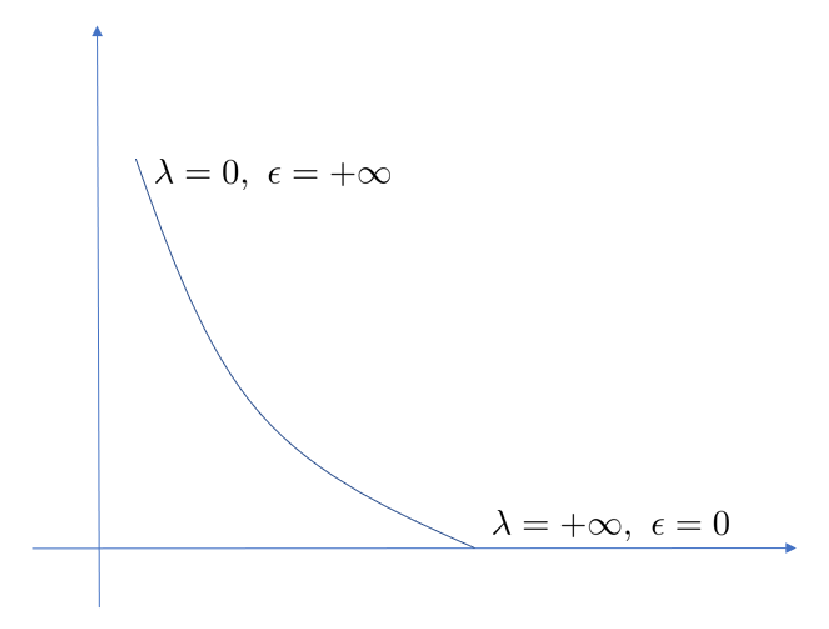
\includegraphics[width=0.5\linewidth]{imgs/ridge.eps}
	\caption{这幅图是目标函数的帕累托曲面,横轴表示最小化误差这一目标,纵轴表示能量这一目标,两个端点分别表示两种表述中的不同取值,例如与横轴的交点,意味着能量为0,即$ \epsilon=0 $,相应的在(1)中代表仅考虑能量,$ \lambda=+\infty $,另一情况同理}
\end{figure}


\end{document}